\documentclass[10pt]{article}
\usepackage[letterpaper,margin=.64in]{geometry}
\usepackage[T1]{fontenc}
\usepackage{lmodern}
\usepackage{microtype}
\usepackage{amsmath,amssymb,booktabs,tabularx,enumitem,multicol}
\usepackage{tikz}
\usetikzlibrary{positioning,arrows.meta}
\usepackage[most]{tcolorbox}
\usepackage{xcolor,hyperref,fancyhdr}
\definecolor{olive}{HTML}{475B3B}\definecolor{gold}{HTML}{986522}\definecolor{teal}{HTML}{236977}\definecolor{cream}{HTML}{F7F7F1}\definecolor{ink}{HTML}{263426}
\hypersetup{colorlinks=true,urlcolor=teal,linkcolor=olive}
\setlength{\parindent}{0pt}\setlength{\parskip}{4.5pt}
\setlist[enumerate]{leftmargin=*,itemsep=4pt,topsep=5pt}
\setlist[itemize]{leftmargin=*,itemsep=3pt,topsep=4pt}
\pagestyle{fancy}\fancyhf{}\lhead{\textcolor{olive}{MATH\& 107 | Module 9}}\rhead{\textcolor{gold}{Computing with Two Choices}}\cfoot{\thepage}\setlength{\headheight}{14pt}
\newtcolorbox{worked}[1]{enhanced,breakable,colback=cream,colframe=olive!55!white,boxrule=.65pt,arc=2mm,title={\bfseries #1},fonttitle=\color{ink},colbacktitle=olive!14!white,coltitle=ink}
\newtcolorbox{taskbox}[1]{enhanced,breakable,colback=white,colframe=gold!75!white,boxrule=.65pt,arc=2mm,title={\bfseries #1},fonttitle=\color{ink},colbacktitle=gold!13!white,coltitle=ink}
\newcommand{\sect}[1]{\medskip\section*{\color{olive}#1}\vspace{-5pt}}
\tikzset{place/.style={draw=olive,very thick,fill=olive!12,rounded corners=2pt,align=center,font=\small,minimum height=8mm,minimum width=19mm},choice/.style={draw=teal,very thick,fill=teal!9,rounded corners=2pt,align=center,font=\small,minimum height=8mm,minimum width=18mm},conn/.style={-Stealth,thick,draw=olive!70}}
\newcommand{\menutree}{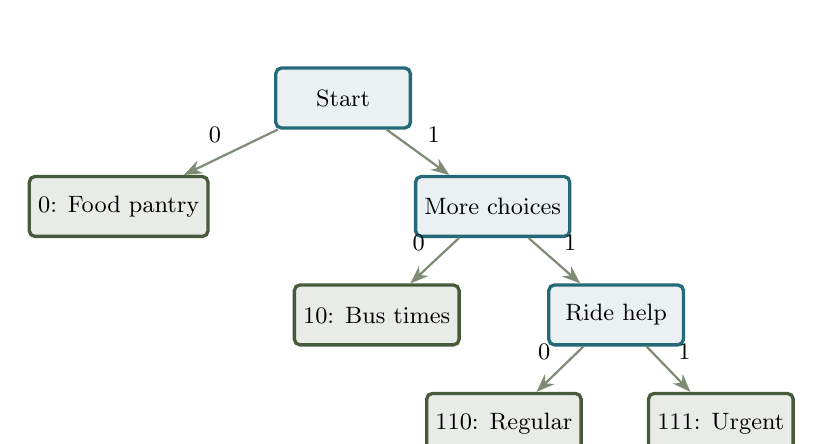
\begin{tikzpicture}[x=1cm,y=1cm,scale=.95,transform shape]
\node[choice] (root) at (0,0) {Start};
\node[place] (food) at (-3,-1.45) {0: Food pantry};
\node[choice] (more) at (2,-1.45) {More choices};
\node[place] (bus) at (.45,-2.9) {10: Bus times};
\node[choice] (ride) at (3.65,-2.9) {Ride help};
\node[place] (reg) at (2.15,-4.35) {110: Regular};
\node[place] (urgent) at (5.05,-4.35) {111: Urgent};
\draw[conn] (root) -- node[above left,font=\small]{0} (food);
\draw[conn] (root) -- node[above right,font=\small]{1} (more);
\draw[conn] (more) -- node[above left,font=\small]{0} (bus);
\draw[conn] (more) -- node[above right,font=\small]{1} (ride);
\draw[conn] (ride) -- node[above left,font=\small]{0} (reg);
\draw[conn] (ride) -- node[above right,font=\small]{1} (urgent);
\end{tikzpicture}}
\newcommand{\addresstree}{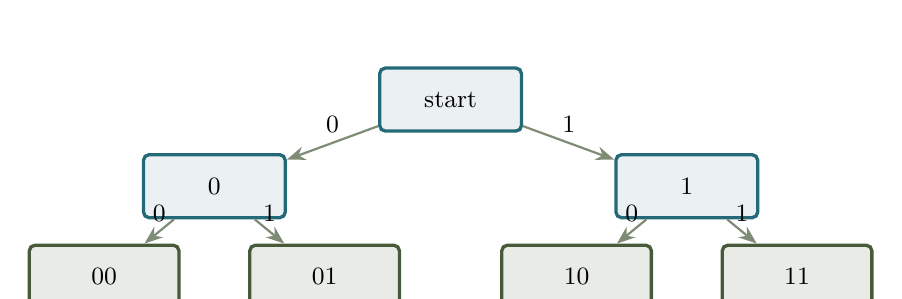
\begin{tikzpicture}[x=1cm,y=1cm]
\node[choice] (r) at (0,0) {start};
\foreach \x/\lab in {-3/0,3/1}{\node[choice] (x\lab) at (\x,-1.1) {\lab};\draw[conn] (r)--node[above,font=\small]{\lab}(x\lab);}
\foreach \x/\p/\lab in {-4.4/0/00,-1.6/0/01,1.6/1/10,4.4/1/11}{\node[place] (y\lab) at (\x,-2.25) {\lab};\draw[conn] (x\p)--node[above,font=\small]{\ifnum\pdfstrcmp{\lab}{00}=0 0\else\ifnum\pdfstrcmp{\lab}{10}=0 0\else 1\fi\fi}(y\lab);}
\end{tikzpicture}}
\begin{document}
{\small\bfseries\color{teal}MATH IN SOCIETY / MODULE 9}\par\vspace{6pt}
{\fontsize{29}{32}\selectfont\bfseries\color{olive}Computing with Two Choices}\par\vspace{5pt}
{\large Binary numbers, decision trees, and short programs}\par\vspace{10pt}
\begin{worked}{A question for the week}
A community center needs to direct callers to the right service. It could ask everyone the same two questions, or it could use a branching menu that takes fewer questions for common requests. How can a few yes-or-no choices describe numbers, routes, and useful instructions?
\end{worked}
We will start by counting with two symbols. Then we will follow branches in a tree, build a small decision program, count the work it requires, and ask what happens when we keep extending the tree. The calculations use counting, addition, and multiplication. You do not need to know how to code.
\sect{1. Counting with zeros and ones}
Our usual decimal system has ten digits. Its positions count ones, tens, hundreds, and so on. The \textbf{binary} system has two digits: 0 and 1. Each position is worth twice the one to its right.
\begin{center}\begin{tabular}{c|ccccc}\toprule Position & 5th & 4th & 3rd & 2nd & 1st\\\midrule Worth & 16 & 8 & 4 & 2 & 1\\\bottomrule\end{tabular}\end{center}
For example, the binary word \texttt{1101} represents $8+4+0+1=13$ in decimal. The leftmost 1 uses the 8's place, the next 1 uses the 4's place, the 0 skips the 2's place, and the last 1 uses the 1's place.
\begin{worked}{From decimal 11 to binary}
Find the largest power of two not exceeding 11: that is 8. We have 3 left, so use 2 and 1 as well. The place values 8, 4, 2, 1 receive digits $1,0,1,1$. Thus $11=1011_2$.
\end{worked}
\begin{taskbox}{Try it}
(a) Find the decimal value of $10110_2$ using the place values $16,8,4,2,1$. (b) Write 14 in binary. (c) How many distinct three-digit strings of zeros and ones are possible if leading zeros are allowed? (Here a \emph{string} is a code, not necessarily the usual way to write a number.)
\end{taskbox}
\sect{2. A code can be a route}
Suppose 0 means ``go left'' and 1 means ``go right.'' Beginning at a dot, each choice follows one branch. A string like \texttt{101} tells you exactly which route to take: right, left, right.
\begin{center}\addresstree\end{center}
The four addresses after two choices are \texttt{00}, \texttt{01}, \texttt{10}, and \texttt{11}. Every additional choice doubles the number of possibilities. With one choice there are 2 addresses; with two there are 4; with three there are 8; with four there are 16. In general, there are $2^n$ binary strings with exactly $n$ digits.
\begin{worked}{Find the address}
The address \texttt{011} means left, then right, then right. The first two digits \texttt{01} bring you to a dot in the two-level tree. A third choice continues from that dot. That first part, \texttt{01}, is called a \textbf{prefix}.
\end{worked}
\begin{taskbox}{Try it}
(a) List all eight three-digit binary addresses. (b) How many four-digit addresses begin with \texttt{10}? (c) Is \texttt{10} a prefix of \texttt{1011}? Is \texttt{11}?
\end{taskbox}
\sect{3. Turning a tree into a program}
A community center answers questions about food pantry hours, bus schedules, regular ride help, and urgent ride help. A caller enters 0 or 1 at each junction and stops when a service appears.
\begin{center}\resizebox{.94\linewidth}{!}{\menutree}\end{center}
This is a \textbf{finite decision program}: follow the branch named by each digit until you arrive at an instruction to stop and show a service. It has four stopping codes:
\begin{center}\begin{tabular}{lcc}\toprule Service & Code & Questions answered\\\midrule Food pantry & \texttt{0} & 1\\Bus times & \texttt{10} & 2\\Regular ride help & \texttt{110} & 3\\Urgent ride help & \texttt{111} & 3\\\bottomrule\end{tabular}\end{center}
Notice that \texttt{0} is never the beginning of another \emph{complete} code. Neither is \texttt{10}. This is a \textbf{prefix-free code}: no stopping code is an initial part of another stopping code. As soon as a caller reaches a service, the system knows the code is complete.
\begin{taskbox}{Try it}
(a) Trace the code \texttt{110}. Which service answers? (b) Why would using \texttt{1} as an additional stopping code cause a problem? (c) Design a new two-question menu for four services, with a distinct two-digit code for each service.
\end{taskbox}
\sect{4. Counting the work a program does}
A decision menu is useful when it answers common requests quickly. Suppose the center receives 16 calls:
\begin{center}\begin{tabular}{lrrr}\toprule Service & Calls & Questions per call & Total questions\\\midrule Food pantry & 8 & 1 & 8\\Bus times & 4 & 2 & 8\\Regular ride help & 2 & 3 & 6\\Urgent ride help & 2 & 3 & 6\\\midrule All calls & 16 && 28\\\bottomrule\end{tabular}\end{center}
The total is $8(1)+4(2)+2(3)+2(3)=28$ questions. If every caller answered exactly two questions, the total would be $16(2)=32$. For this group of callers, the branching menu saves four questions.
\begin{worked}{Same tree, different callers}
A different community center might receive urgent requests most often. The tree's shape can stay the same while the service labels change. Assigning the shortest code to the most frequent request changes how much work the menu does.
\end{worked}
\begin{taskbox}{Try it}
Suppose the call counts are 6 for food pantry, 5 for bus times, 3 for regular ride help, and 2 for urgent help. How many questions does the current menu ask in total? How many would a two-question menu ask? Which one uses fewer questions?
\end{taskbox}
\sect{5. A tree that keeps growing}
A decision program can stop after a few choices. But we can also imagine a binary tree with no final level: every address has two longer addresses beneath it, one ending in 0 and one ending in 1. A three-digit address is a location \emph{within} that tree, not the end of the whole tree.
\begin{center}\begin{tabular}{c|rrrrr}\toprule Choices made & 0 & 1 & 2 & 3 & 4\\\midrule Possible addresses & 1 & 2 & 4 & 8 & 16\\\bottomrule\end{tabular}\end{center}
An \textbf{infinite path} would be a never-ending sequence of choices. At any finite stage we know only its beginning, called a \textbf{finite prefix}. For example, after seeing \texttt{101}, the next digit could be 0 or 1. Both paths agree on everything observed so far.
\begin{worked}{A rule removes some possibilities}
Imagine a code that never uses two 1s together. The allowed two-digit strings are \texttt{00}, \texttt{01}, and \texttt{10}. The string \texttt{11} is forbidden. At three digits, the allowed strings are \texttt{000}, \texttt{001}, \texttt{010}, \texttt{100}, \texttt{101}: five addresses. At four digits there are eight.
\end{worked}
\begin{taskbox}{Try it}
(a) List the allowable three-digit strings that begin with 1. (b) Write two allowed four-digit strings and one forbidden four-digit string. (c) Without listing everything, explain why every allowed string ending in 1 must be followed by 0 if we extend it one step.
\end{taskbox}
A finite decision tree is one kind of program: it makes choices and stops after a bounded number of questions. Real programs can also repeat instructions in loops. A short program can therefore do a very long calculation. That distinction is one reason the study of computation is interesting.
\sect{6. What have we discovered?}
Binary digits can stand for numbers or for instructions. The meaning comes from the rule we choose. In a decision tree, a code is a path. A stopping instruction makes the tree into a simple program. By counting the paths and questions, we can compare how much work different designs require. Even a short rule can organize an ever-growing set of possible routes.
\begin{worked}{One reliable way to investigate a decision program}
(1) Say what each choice means. (2) Trace the path for a particular input. (3) Identify when the process stops. (4) Count the questions or possible outcomes. (5) Explain one detail that the model leaves out.
\end{worked}
\sect{Practice}
\begin{enumerate}
\item Convert $11010_2$ to decimal. Write 9 in binary.
\item How many addresses have exactly five binary digits? How many of them begin with \texttt{011}?
\item In the menu above, which code reaches urgent ride help? Why can the code \texttt{1} not also mean ``stop''?
\item A desk receives 10 pantry requests, 3 bus requests, 2 regular ride requests, and 1 urgent request. Count the total questions using the menu above. Compare with a fixed two-question menu.
\item List all allowed two-digit and three-digit codes that avoid \texttt{11}. Explain why the number is smaller than $2^n$.
\item Describe a useful decision tree from daily life. Name one thing the tree would need to know that is not represented by a simple yes-or-no choice.
\end{enumerate}
\begin{worked}{Answers to calculation questions}
1. $11010_2=16+8+2=26$ and $9=1001_2$. 2. $2^5=32$ total; four begin with \texttt{011} because two positions remain free. 3. \texttt{111}; stopping at \texttt{1} would prevent distinguishing the three codes that begin with 1. 4. $10(1)+3(2)+2(3)+1(3)=25$ questions, versus $16(2)=32$. 5. Two digits: \texttt{00}, \texttt{01}, \texttt{10}; three: \texttt{000}, \texttt{001}, \texttt{010}, \texttt{100}, \texttt{101}. The rule removes all addresses with adjacent 1s. 6. Answers vary.
\end{worked}
\end{document}
